\documentclass[../besoin_user.tex]{subfiles}
\begin{document}
\section{Connexion}
\begin{figure}[h]
    \centering
    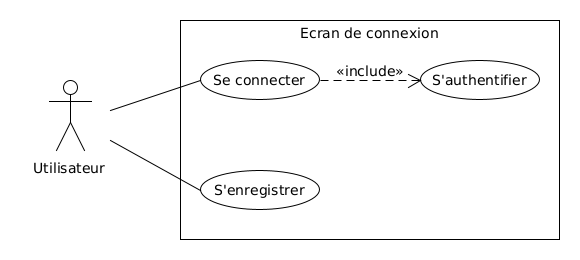
\includegraphics[scale=0.6]{img_fonctionnel/use_case_user_connexion.png}
    \label{fig:user_connexion}
    \caption{Connexion}
\end{figure}
  Lorsque le jeu est lancé, une fenêtre de connexion s'affiche, offrant à l'utilisateur la possibilité de se connecter à son compte. 
  Si l'utilisateur ne dispose pas encore d'un compte, il a la possibilité d'en créer un. 
  En cas de saisie de données incorrectes, le programme informe l'utilisateur de l'erreur. 
  Une fois l'authentification réussie, l'utilisateur est dirigé vers le menu principal du jeu.
  \newpage
\end{document}